\section{Simulation experiments}
\label{sec:supp_execution}
\subsection{Helsinki response through assignment and routing}
\label{sec:execution_revision}
The Helsinki experiment uses a fixed population of 1,000 travelers with fixed origin--destination pairs, HSL timetables and an OSM road network. The perceived-delay condition changes the input to the behavioral model while the physical timetable stays the same. Table~\ref{tab:execution_design} summarizes the fitted models, assignment rules and paired comparisons. The soft-KL and direction+magnitude Students are the three models per objective selected by validation KL, and MNL-S is combined with each of its three independently trained neural timing predictors.

PT use is traced through predicted probabilities, feasibility-adjusted probabilities, assigned modes, routed modes and simulated boarding, with records matched by person. A traveler counts as a simulated PT user after boarding a PT vehicle before the outbound destination, whether or not the journey is later completed. All responses use the same 1,000 people as denominator, whereas the share of assigned PT users who board is computed over the number assigned to PT. Completion, boardings and legs are reported as separate outcomes. Table~\ref{tab:execution_layers} gives every intermediate stage, and Table~\ref{tab:execution_gap_aggregation} contrasts signed averages with absolute gaps.
\begin{table}[pos=htbp]
\centering\small
\caption{Design of the Helsinki simulation experiment.}
\label{tab:execution_design}
\begin{tabular*}{\linewidth}{@{\extracolsep{\fill}}ll@{}}
\toprule
Quantity & Configuration \\
\midrule
Initial population & 1,000 fixed people and OD pairs \\
Conditions & Baseline and 15-minute perceived-delay input; physical timetable fixed \\
Fitted models & 10: SA-Student; three each of soft KL, direction+magnitude and MNL-S with timing \\
Assignment rules & Deterministic, stochastic, and feasibility-constrained stochastic assignment \\
Assignment seeds & 42, 2026 and 7, with common draws across paired conditions \\
Runs & 14 per fitted model; 140 runs, 70 paired baseline--delay comparisons \\
Simulation & Flow and storage capacity factors of 0.3; one MATSim iteration \\
\bottomrule
\end{tabular*}
\par\smallskip{\footnotesize Walking and cycling trips use speeds derived from the road links. Walking legs outside the network, such as access to stops, use 1.39 m/s.}
\end{table}

\begin{table}[pos=htbp]
\centering\small
\caption{Helsinki PT responses at every stage from prediction to simulation, averaged over assignment repetitions within each fitted model and then over models.}
\label{tab:execution_layers}
\setlength{\tabcolsep}{3pt}
\renewcommand{\arraystretch}{1.12}
\begin{tabular*}{\linewidth}{@{\extracolsep{\fill}}llrrrrr@{}}
\toprule
Model & Assignment & Predicted & Adjusted & Assigned & Routed & Simulated \\
\midrule
Direction+magnitude & Constrained & -6.77 & -6.84 & -7.22 & -7.22 & -7.22 \\
Direction+magnitude & Deterministic & -6.77 & -6.77 & -8.10 & -8.63 & -8.63 \\
Direction+magnitude & Stochastic & -6.77 & -6.77 & -7.01 & -7.12 & -7.12 \\
MNL-S + neural time & Constrained & -6.84 & -6.10 & -6.67 & -6.67 & -6.67 \\
MNL-S + neural time & Deterministic & -6.84 & -6.84 & -7.30 & -6.90 & -6.90 \\
MNL-S + neural time & Stochastic & -6.84 & -6.84 & -7.40 & -6.63 & -6.63 \\
SA-Student & Constrained & -13.10 & -12.83 & -14.17 & -14.17 & -14.17 \\
SA-Student & Deterministic & -13.10 & -13.10 & -13.00 & -12.30 & -12.30 \\
SA-Student & Stochastic & -13.10 & -13.10 & -14.60 & -14.17 & -14.17 \\
Soft KL & Constrained & -6.97 & -6.60 & -7.06 & -7.06 & -7.06 \\
Soft KL & Deterministic & -6.97 & -6.97 & -7.60 & -8.03 & -8.03 \\
Soft KL & Stochastic & -6.97 & -6.97 & -7.34 & -6.97 & -6.97 \\
\bottomrule
\end{tabular*}
\par\smallskip{\footnotesize All entries are percentage points with the same 1,000 initial people per run. The main table separates training variation from sampling variation. Results for individual runs are given in the supplementary data files.}
\end{table}

\begin{table}[pos=htbp]
\centering\small
\caption{Cancellation of signed gaps between predicted and simulated responses in Helsinki.}
\label{tab:execution_gap_aggregation}
\setlength{\tabcolsep}{3pt}
\renewcommand{\arraystretch}{1.12}
\begin{tabular*}{\linewidth}{@{\extracolsep{\fill}}llrrrrr@{}}
\toprule
Model & Policy & Models & Pairs & $|\overline{g}|$ & $\overline{|\bar g_m|}$ & $\overline{|g_{ms}|}$ \\
\midrule
SA-Student & Deterministic & 1 & 1 & 0.795 & 0.795 & 0.795 \\
SA-Student & Stochastic & 1 & 3 & 1.072 & 1.072 & 1.402 \\
SA-Student & Constrained & 1 & 3 & 1.072 & 1.072 & 1.268 \\
Soft KL & Deterministic & 3 & 3 & 1.061 & 1.179 & 1.179 \\
Soft KL & Stochastic & 3 & 9 & 0.005 & 1.453 & 1.508 \\
Soft KL & Constrained & 3 & 9 & 0.084 & 1.380 & 1.419 \\
Direction+magnitude & Deterministic & 3 & 3 & 1.865 & 1.865 & 1.865 \\
Direction+magnitude & Stochastic & 3 & 9 & 0.354 & 0.906 & 0.961 \\
Direction+magnitude & Constrained & 3 & 9 & 0.454 & 0.872 & 0.883 \\
MNL-S + neural time & Deterministic & 3 & 3 & 0.061 & 0.061 & 0.061 \\
MNL-S + neural time & Stochastic & 3 & 9 & 0.206 & 0.206 & 0.780 \\
MNL-S + neural time & Constrained & 3 & 9 & 0.173 & 0.173 & 0.813 \\
\bottomrule
\end{tabular*}
\par\smallskip{\footnotesize All gaps are simulated minus predicted response, in percentage points. The first measure takes the absolute value after averaging signed gaps across sampling and training seeds. The second first averages sampling within each fitted model, then averages the absolute model gaps. The third averages absolute gaps over all baseline--delay run pairs. Opposite signed gaps can cancel only in the first measure across models; sampling effects can additionally cancel within the second. All three are summaries of the same runs.}
\end{table}

Trips are routed at the departure time adjusted by each model. For SA-Student, routing at the adjusted rather than the desired departure time changes the itinerary of 279 travelers at baseline and 313 under delay, while the same 684 people have a feasible PT route at both departure times in each condition. Itineraries can thus change without any change in feasibility. The supplementary data files list all 70 baseline--delay comparisons with their paired-person intervals, at the precision reported in the tables. Section~\ref{sec:materials_scope} describes which details of the routing procedure these summaries document.
\FloatBarrier

\subsection{Active-mode speed sensitivity in Shanghai}
\label{sec:speed_sensitivity}
The Shanghai experiment holds the 321 people, their assigned modes, departure times and plans fixed, and compares active-mode speeds derived from the network links with caps of 1.34 m/s for walking and 4.17 m/s for cycling. The timetable is the same in the baseline and perceived-delay conditions. PT users number 224 at baseline and 134 under delay, and every person completes both journeys.

With network-derived speeds, mean outbound times are 19.68 minutes at baseline and 15.23 minutes under perceived delay. With speed caps, the corresponding means are 33.59 and 47.63 minutes. The paired difference is therefore $-4.44$ minutes ($[-5.06,-3.84]$) under link speeds and $+14.04$ minutes ($[11.18,17.05]$) under speed caps (Figure~\ref{fig:speed_sensitivity}). Delay moves 90 travelers away from PT, and whether this shortens or lengthens the average journey depends on the speeds assumed for walking and cycling. The times are model outputs and have not been compared with observed trip durations.
\begin{figure}[pos=htbp]
\centering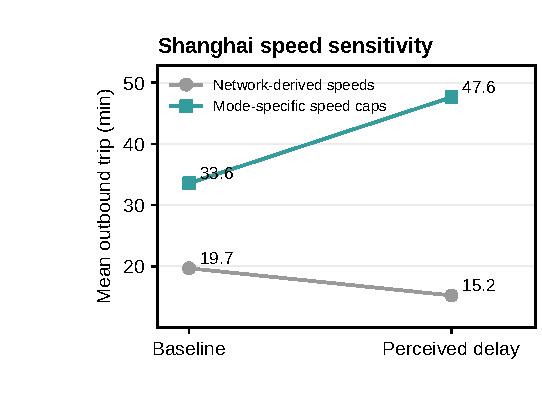
\includegraphics[width=.57\textwidth]{figures/narrative/figureS_speed_sensitivity.pdf}
\caption{Sensitivity of Shanghai journey times to the speeds of walking and cycling in the simulation. People, assigned modes, departure times and physical timetables are identical across speed settings. Values are mean durations of completed outbound trips.}
\label{fig:speed_sensitivity}
\end{figure}

\subsection{Singapore population responses and journey measures}
The Singapore scenario experiment simulates 10,000 synthetic travelers on unchanged physical supply. Scenario C0 is the baseline, C1 introduces heavy rain, C2 a 50\% fare increase and C3 a perceived PT delay of 15 minutes. C4 represents a road disruption that adds 20 minutes of car travel time and 20 minutes of reliability delay, and C5 combines rain with PT delay. Populations drawn with seeds 2026, 42 and 7 vary the composition of travelers, and MATSim uses seed 4711. Table~\ref{tab:singapore} gives the exact shares shown in Figure~\ref{main-fig:concept} of the main article, and Table~\ref{tab:seeds} their sensitivity to population composition.
\begin{table}[pos=htbp]
\centering\small
\setlength{\tabcolsep}{3pt}
\caption{Singapore absolute Student decision shares (percent) and MATSim consequences. Time is the completed-leg mean, not the mean journey duration per person. Seed 2026, 10,000 agents.}
\label{tab:singapore}
\begin{tabular}{@{}lrrrrrrr@{}}
\toprule
Scenario & Car & PT & Bike & Walk & Boardings & Car VKT (km) & \shortstack{Completed-leg\\mean (min)} \\
\midrule
C0 & 28.3 & 25.3 & 34.0 & 12.4 & 5613 & 33,939.0 & 43.67 \\
C1 & 37.6 & 45.3 & 13.3 & 3.8 & 9761 & 42,777.5 & 50.86 \\
C2 & 29.9 & 25.7 & 32.6 & 11.8 & 5674 & 35,797.8 & 43.86 \\
C3 & 29.0 & 10.3 & 35.8 & 25.0 & 2474 & 34,684.6 & 32.23 \\
C4 & 1.8 & 37.5 & 41.8 & 19.0 & 8537 & 2,943.4 & 52.71 \\
C5 & 37.7 & 18.6 & 24.5 & 19.2 & 4301 & 42,822.8 & 38.27 \\
\bottomrule
\end{tabular}
\end{table}

\begin{table}[pos=htbp]
\centering\small
\caption{Paired population-seed responses from the existing multi-seed summary.}
\label{tab:seeds}
\begin{tabular}{@{}lrrr@{}}
\toprule
Scenario & Seed & $\Delta$ PT pp & $\Delta$ car pp \\
\midrule
C1 & 2026 & +20.0 & +9.3 \\
C1 & 42 & +19.7 & +9.2 \\
C1 & 7 & +20.1 & +9.2 \\
C2 & 2026 & +0.4 & +1.6 \\
C2 & 42 & +0.5 & +1.8 \\
C2 & 7 & +0.5 & +1.5 \\
C3 & 2026 & -15.1 & +0.8 \\
C3 & 42 & -15.3 & +0.6 \\
C3 & 7 & -15.7 & +0.6 \\
C4 & 2026 & +12.1 & -26.5 \\
C4 & 42 & +11.7 & -26.1 \\
C4 & 7 & +12.3 & -26.5 \\
C5 & 2026 & -6.7 & +9.4 \\
C5 & 42 & -6.4 & +9.3 \\
C5 & 7 & -6.9 & +9.1 \\
\bottomrule
\end{tabular}
\end{table}

Journey measures for each person run from the first departure to the first activity other than home or an interaction point created by routing, such as a transfer. Table~\ref{tab:singapore_person_counts} reports people, boardings and legs separately. At baseline, 9,741 people complete the outbound journey and 9,062 return home. A completed outbound journey takes 66.43 minutes on average, whereas a completed leg takes 43.67 minutes, because a PT journey can consist of several legs.

Table~\ref{tab:singapore_person_time} also reports, for every departing person, the time elapsed until completion or until the end of the 30-hour simulation, a descriptive measure that includes unfinished journeys. Paired differences between scenarios use people who complete both trips and 4,000 paired-person resamples. All times reflect the network-based speeds and the fixed supply.
\begin{table}[pos=htbp]
\centering\footnotesize
\caption{Person and leg counts across six Singapore scenarios.}
\label{tab:singapore_person_counts}
\setlength{\tabcolsep}{3pt}
\renewcommand{\arraystretch}{1.15}
\begin{tabular}{@{}lrrrrrrr@{}}
\toprule
Scenario & \shortstack{Outbound\\complete} & \shortstack{Return\\complete} & \shortstack{Outbound\\PT people} & Boardings & \shortstack{Unfinished\\legs} & \shortstack{Stuck\\people} & \shortstack{Completed\\legs} \\
\midrule
C0 & 9,741 & 9,062 & 2,456 & 5,613 & 938 & 211 & 29,476 \\
C1 & 9,546 & 8,367 & 4,442 & 9,761 & 1,633 & 366 & 36,477 \\
C2 & 9,730 & 9,044 & 2,492 & 5,674 & 956 & 221 & 29,567 \\
C3 & 9,884 & 9,600 & 961 & 2,474 & 400 & 102 & 24,219 \\
C4 & 9,647 & 8,619 & 3,671 & 8,537 & 1,381 & 285 & 34,499 \\
C5 & 9,789 & 9,268 & 1,779 & 4,301 & 732 & 183 & 27,266 \\
\bottomrule
\end{tabular}
\par\smallskip\begin{minipage}{0.98\textwidth}\footnotesize Each scenario starts with and departs all 10,000 people. Completion and PT use are person counts. Boardings include transfers and both travel directions; unfinished legs and completed legs are different event-level counts. A stuck person may also have an unfinished leg.\end{minipage}
\end{table}

\begin{table}[pos=htbp]
\centering\footnotesize
\caption{Singapore timing with explicit units and completion conditions. All times are in minutes.}
\label{tab:singapore_person_time}
\setlength{\tabcolsep}{3pt}
\renewcommand{\arraystretch}{1.15}
\begin{tabular}{@{}lrrrrrl@{}}
\toprule
Scenario & \shortstack{Completed-leg\\mean} & \shortstack{Outbound\\mean} & \shortstack{Outbound\\median} & \shortstack{Completion-or-\\horizon mean} & \shortstack{Paired\\people} & \shortstack{Paired outbound change\\versus C0 [95\% CI]} \\
\midrule
C0 & 43.67 & 66.43 & 17.45 & 88.80 & -- & -- \\
C1 & 50.86 & 98.50 & 20.19 & 135.60 & 9,511 & +32.00 [+29.17, +34.69] \\
C2 & 43.86 & 66.88 & 16.97 & 90.01 & 9,708 & +0.60 [-0.45, +1.69] \\
C3 & 32.23 & 38.92 & 15.67 & 49.78 & 9,724 & -27.68 [-29.86, -25.56] \\
C4 & 52.71 & 94.78 & 27.08 & 124.21 & 9,578 & +28.39 [+25.98, +30.83] \\
C5 & 38.27 & 53.33 & 14.35 & 71.97 & 9,695 & -13.87 [-15.83, -11.96] \\
\bottomrule
\end{tabular}
\par\smallskip\begin{minipage}{0.98\textwidth}\footnotesize Outbound means and medians condition on the scenario-specific completers in Table~\ref{tab:singapore_person_counts}; the horizon mean retains all 10,000 departed people until completion or the administrative end at simulation hour 30. Paired changes retain only people completing both outbound journeys and use 4,000 paired-person bootstrap resamples (seed 917). The link-speed implementation limits interpretation as calibrated travel time.\end{minipage}
\end{table}

\FloatBarrier

\subsection{Feasibility correction and response geometry}
\label{sec:feasibility_geometry}
For a normalized distribution $\mathbf p$ and feasible set $F$ with mass $Z>0$, conditional renormalization adds mass $1-Z$ within $F$ and removes mass $1-Z$ outside it. Hence $\|\mathbf q-\mathbf p\|_1=2(1-Z)$. Every distribution supported on $F$ must remove all outside mass, and its inside changes have a sum of $1-Z$; the triangle inequality therefore gives the same lower bound. Conditional renormalization attains it, though the $L_1$ minimizer need not be unique.

An endpoint-optimal correction need not preserve a paired response. For a fixed feasible set $F=\{1,2\}$, let baseline probabilities be $(0.4,0.3,0.3)$ and perturbed probabilities $(0.4,0.2,0.4)$. Their corrections are $(4/7,3/7,0)$ and $(2/3,1/3,0)$. The probability of mode 1 is unchanged before correction but increases by $2/21$ afterward. This constructed example proves the distinction without making a claim about its empirical prevalence. The main-text decomposition reports the specified correction separately from subsequent execution; it does not attribute every correction-induced response difference to an unavoidable lower bound.
\FloatBarrier
